\chapter{紫外發散與超對稱的解決之道}

\lectureoverview{在引入超對稱的形式數學之前，我們應先確切說明它要解決什麼問題。我們會分別在位置空間與動量空間描述紫外發散，透過量綱分析推導標量與費米子傳播子的短距離行為，並估算標量質量的領先圈修正。標量圈與費米子圈對截止尺度的二次依賴相同，但符號相反。若要讓這種抵消來自結構而非偶然，就得追問有什麼原理能使兩者的耦合、多重度與質量充分匹配；超對稱的說服力正是在這個問題上顯現。}

\section{為什麼要重新討論發散？}

原本打算立即開始介紹超對稱的數學架構。不過，最好先把抽象內容延後一講，重新建立其動機。先前對發散與質量重整化的說明過於匆促；若不先看清楚究竟需要修正什麼，超對稱就會像是任意發明的數學構造。

費曼圖在粒子物理學中有兩種密切相關的用途。最常見的是用來整理散射振幅：我們指定入射與出射粒子，再將所需階數的所有圖所代表的振幅加總。費曼圖也用來構造\emph{有效拉格朗日量}。此處的``有效''不是稱讚它特別成功，而是表示這種描述只是一種近似：無法探測的短距離細節已被消去或積分掉，其影響則編碼在留下來的參數與相互作用中。

每種這樣的描述都有其適用範圍。我們可以用最短的可信距離來界定這個範圍，記作\(\delta\)；也可以用最大的可信動量來界定：
\begin{equation}
\Lambda\sim \delta^{-1}.
\end{equation}
這兩種截止並非彼此獨立的假設，而是同一紫外極限的傅立葉對偶描述。

\section{一個傳播子，兩種描述}

傳播子是粒子在一個時空點被產生或插入，並在另一個時空點被移除或探測到的振幅。令這兩個點為\(x^\mu\)與\(y^\mu\)，並將兩點間的間隔寫作
\begin{equation}
\Delta^\mu=y^\mu-x^\mu.
\end{equation}
我們用小寫符號\(\delta\)表示截止尺度，以免和兩點間的間隔混淆。

平移不變性表示，自由傳播子對\(x\)與\(y\)的依賴只透過\(\Delta\)呈現。同一個量也可以作傅立葉變換：
\begin{equation}
G(\Delta)
=\int\frac{d^4k}{(2\pi)^4}\,e^{-ik\cdot\Delta}\,\widetilde G(k).
\end{equation}

向聽眾提出``位置的傅立葉共軛量是什麼？''時，答案是動量。因此，在位置空間中，圈圖可描述為傳播子返回起點；在動量空間中，則等價地描述為對所有可能繞圈傳遞的動量積分。動量空間的規則要求在每個頂點施加動量守恆；位置空間則讓目前的冪次計數論證更清楚。

在進行任何計算之前，這種等價性已指出紫外問題所在。在位置空間中，圈圖探測的是兩點重合的極限\(\Delta\to0\)；在動量空間中，則探測\(|k|\to\infty\)的極限。大動量對應短波長，因此短距離奇異性與高動量發散，只是同一現象在不同座標下的呈現。

本講討論最簡單的幾種自旋類別：標量場、費米子場，以及作為背景的規範場。標量的自旋為零，以單分量場\(\phi(x)\)表示。2010年錄製本講時，希格斯粒子尚未被發現，當時被描述為粒子物理學中預期存在的主要標量。這段歷史背景說明了戲稱``希格斯威格斯''的由來：這個場在物理上備受關注，但當時尚未獲得實驗證實。

對實標量場而言，傳播子可示意性地寫成
\begin{equation}
G_\phi(x,y)=\expect{0|T\!\left\{\phi(x)\phi(y)\right\}|0}
=G_\phi(\Delta).
\end{equation}
時間排序的慣例與正規化不影響冪次計數。重要的是，這兩個場的插入分別描述粒子在一點被產生，以及在另一點被湮滅。

\begin{classroomqa}
\audiencequestion{\(x\)和\(y\)是空間中的位置，還是時空中的位置？\lecturetimestamp{00:09:31}}
\lecturerresponse{它們是時空點，各自都是四向量。因此，傳播子取決於兩點間的四維間隔；在洛倫茲不變的真空中，它取決於相應的不變間隔。}
\end{classroomqa}

自旋為二分之一的粒子以狄拉克場\(\psi_i(x)\)描述。指標\(i\)是旋量指標，不是空間分量，因此傳播子是矩陣：
\begin{equation}
S_{ij}(x,y)=\expect{0|T\!\left\{\psi_i(x)\bar\psi_j(y)\right\}|0}
=S_{ij}(\Delta).
\end{equation}

向聽眾提出的一個問題給出了分量數：四維狄拉克場有四個複數分量。無質量的外爾場可用兩個複數分量描述，因此左手場與右手場可以分開處理。就目前的量綱論證而言，只要知道傳播子具有旋量矩陣結構即可。

由於\(S_{ij}\)是\(4\times4\)矩陣，可以將它按狄拉克矩陣的基底展開。我們先略去這些指標，等到需要時再寫回來。這不是說矩陣結構不存在，而是在建立紫外冪律時刻意採取的簡化。

\begin{classroomqa}
\audiencequestion{傳播子中何時必須出現共軛場或厄米共軛場？\lecturetimestamp{00:14:06}}
\lecturerresponse{在這個示意性討論中，實的中性標量場由同一個場包含產生與湮滅算符，因此不需要另外引入厄米共軛場。對於帶電場，則必須區分粒子與反粒子的算符。因此，對電子而言，\(\psi\)、\(\psi^\dagger\)與其協變形式\(\bar\psi=\psi^\dagger\gamma^0\)扮演不同的角色。}
\end{classroomqa}

希格斯粒子本身是電中性的，儘管標準模型中的希格斯場是電弱二重態。本講以實的中性標量作為局部模型；對紫外估算來說，這項簡化已經足夠。\editorialnote{這項區分可避免把示意性的實標量例子誤認為對電弱希格斯多重態的完整描述。}

\section{自然單位與標量場的量綱}

令\(\hbar=c=1\)。於是長度與時間的單位相同，而能量、質量與動量的量綱都是長度的倒數：
\begin{equation}
[m]=[E]=[p]=L^{-1}.
\end{equation}
作用量出現在相位\(e^{iS}\)中，因此是無量綱的。四維時空中，一個典型的標量作用量為
\begin{equation}
S_\phi=\int d^4x\left[
\frac12\partial_\mu\phi\,\partial^\mu\phi
-\frac12m^2\phi^2
-\frac{\lambda}{4!}\phi^4
+\cdots\right].
\end{equation}
慣用的因子\(1/2\)與\(1/4!\)不影響量綱分析。

先看動能項。由於\([d^4x]=L^4\)與\([\partial_\mu]=L^{-1}\)，無量綱條件給出
\begin{align}
1
&=L^4\left(L^{-1}[\phi]\right)^2,\\
[\phi]&=L^{-1}.
\end{align}
質量項也可用來檢查：
\begin{equation}
L^4[m^2][\phi^2]
=L^4L^{-2}L^{-2}=1.
\end{equation}

接著向聽眾提出的問題是四次耦合的量綱。在四維時空中，它是無量綱的：
\begin{equation}
L^4[\lambda][\phi]^4=L^4[\lambda]L^{-4}=1
\quad\Longrightarrow\quad [\lambda]=L^0.
\end{equation}
因此，\(\phi^4\)相互作用在四維中特別。\(\phi^6\)及更高次相互作用的量綱也遵循同一規則，但其耦合帶有質量的負次冪，表示它們在有效理論中的適用範圍較受限制。

因此，只看場的量綱，就能知道哪些相互作用可以帶有無量綱係數。同樣的方法也能求出傳播子與湯川耦合的量綱，無須計算詳細的費曼積分。

\section{短距離下的標量傳播子}

先考慮無質量標量。它沒有內在長度尺度，因此唯一可用的尺度就是間隔\(\Delta\)。平移不變性表示依賴只透過\(\Delta\)呈現；洛倫茲不變性則將其限制為依賴不變模長。兩個標量場的乘積具有\(L^{-2}\)的量綱。因此，略去數值常數後，
\begin{equation}
G_0(\Delta)\sim\frac{1}{\Delta^2}.
\end{equation}
僅憑量綱分析無法決定\(4\pi^2\)等因子。

質量引入康普頓長度\(m^{-1}\)。從色散關係可以最容易看出它的影響：
\begin{equation}
E=\sqrt{\bm p^{,2}+m^2},
\qquad
E=|\bm p|\quad(m=0).
\end{equation}
當\(|\bm p|\gg m\)時，質量可以忽略。高動量探測的是短距離，因此當\(\Delta\to0\)時，有質量的傳播子必須趨近無質量傳播子的\(1/\Delta^2\)行為。距離遠大於\(m^{-1}\)時，傳播會受到抑制。講座以此式示意：
\begin{equation}
G_m(\Delta)\sim \frac{e^{-m|\Delta|}}{\Delta^2}.
\end{equation}
這刻意不是精確公式。在四維歐幾里得空間中，精確的自由傳播子正比於\(mK_1(mr)/r\)，其中\(r=|\Delta|\)；它具有相同的\(1/r^2\)紫外奇異性，並在長距離呈指數衰減，另帶有冪律前因子。\editorialnote{貝塞爾函數形式是講座中示意性指數衰減的標準精確表述，但冪次計數不需要用到它。}

關鍵之處很簡單：質量會抑制長距離傳播，卻無法消除兩點重合處的奇異性。靠近一點到足夠程度時，任何有限質量都變得無關緊要。

\section{標量蝌蚪圖與精細調節}

四次相互作用\(\lambda\phi^4\)會產生一個有四條線的頂點。將其中兩條線彼此接起來，另外兩條標量線則留作外線，就得到蝌蚪圖。這個圖修正\(\phi^2\)的係數，也就是標量質量平方的係數。

保留的畫面正好呈現了從量綱分析轉向圈修正的時刻。色散關係仍在左側，標量作用量與場的量綱仍部分顯示於右側，而中央剛出現一個小蝌蚪圖。

\begin{figure}[H]
\centering
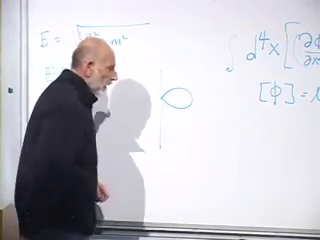
\includegraphics[width=0.72\textwidth]{lecture_03_figure_02.png}
\lectureframe{00:28:30.560}

\medskip
\begin{tikzpicture}[line width=0.8pt,scale=1.0]
  \draw[dashed] (-2.6,0) -- (0,0) -- (2.6,0);
  \fill (0,0) circle (0.055);
  \draw (0,0) .. controls (-0.85,0.7) and (-0.85,1.6) .. (0,1.6)
                .. controls (0.85,1.6) and (0.85,0.7) .. (0,0);
\end{tikzpicture}
\caption{標量自能推導過程中的黑板畫面，以及隨後對蝌蚪圖拓樸所作的保守示意重繪。截圖可清楚確認圈圖、相對論性與無質量能量公式，以及部分作用量；被遮住的係數與標示無法確認，因此不予呈現。}
\end{figure}

在頂點處，標量可以被吸收再發射，另外兩條線則從該點傳播後回到同一點。略去數值與組合因子，修正為
\begin{equation}
\delta m_\phi^2\sim \lambda G_\phi(0).
\end{equation}
在連續理論近似下，重合點的傳播子是無限大。有效理論不宣稱在任意短距離都適用，因此施加\(|\Delta|\geq\delta\)。於是
\begin{equation}
G_\phi(0)\longrightarrow G_\phi(\delta)sim\frac{1}{\delta^2},
\qquad
\delta m_\phi^2\sim\frac{\lambda}{\delta^2}sim\lambda\Lambda^2.
\end{equation}
這稱為二次發散，因為其中含有動量截止的二次方。動量空間的積分也會導出相同結論：過大的貢獻來自任意大的圈動量。最短尺度最終由大統一、量子重力，或尚未想到的其他物理設定，都不影響這項有效理論的判斷。

這就是精細調節問題。如果\(\delta\)極小，而\(\lambda\)並未小到異常的程度，輻射修正就會遠大於低能下觀測到的標量質量平方。如此一來，裸係數與圈修正必須精確抵消到許多位數，令人難以置信：
\begin{equation}
m_{\mathrm{physical}}^2
=m_{\mathrm{bare}}^2+\delta m_\phi^2.
\end{equation}
有質量傳播子也無法挽救這個情況。在造成發散的距離上，\(e^{-m|\Delta|}\simeq1\)。紫外圈圖在到達截止尺度之前，就早已不受質量影響。

\section{費米子的量綱與傳播子}

現在以相同的量綱分析處理狄拉克費米子。其自由作用量為
\begin{equation}
S_\psi=\int d^4x\,
\bar\psi\left(i\gamma^\mu\partial_\mu-m\right)\psi.
\end{equation}
伽馬矩陣是數值矩陣，且無量綱。動能項只含一個導數，因此
\begin{align}
1
&=L^4[\bar\psi]L^{-1}[\psi],\\
[\psi]=[\bar\psi]&=L^{-3/2}.
\end{align}
半整數次冪不必令人擔心；費米子在許多地方都會帶來半整數。

\begin{classroomqa}
\audiencequestion{從質量項推導\([\psi]\)不是比較簡單嗎？\lecturetimestamp{00:36:02}}
\lecturerresponse{是的。質量項給出\(L^4L^{-1}[\bar\psi\psi]=1\)，因此\([\bar\psi\psi]=L^{-3}\)，也就得到\([\psi]=L^{-3/2}\)。先從動能項推導，是因為這種推導在無質量理論中仍然適用，也能顯示為什麼費米子質量以\(m\)而非\(m^2\)的形式出現。}
\end{classroomqa}

兩個費米子場的乘積具有\(L^{-3}\)的量綱，因此講義以簡潔的量綱記號將無質量傳播子寫成
\begin{equation}
S(\Delta)\sim\frac{1}{|\Delta|^3}.
\end{equation}
恢復其矩陣結構後，洛倫茲協變性要求分子具有更精確的形式：
\begin{equation}
S_{ij}(\Delta)
\propto
\frac{\left(\gamma_\mu\Delta^\mu\right)_{ij}}
{\left(\Delta^2\right)^2}.
\end{equation}
分子多出一個長度冪次，因此分母含有間隔的四次方；整體量綱仍為\(L^{-3}\)。和標量情形一樣，費米子質量會抑制大間隔處的傳播，但不改變短距離的尺度行為。

\section{為什麼閉合費米子圈帶負號}

現在可以問，費米子圖能否抵消有問題的玻色子自能。標量蝌蚪圖的符號為正，至多乘上\(\pi\)的冪次或組合係數等正數值因子。閉合費米子圈則帶有相反的符號。

\begin{classroomqa}
\audiencequestion{費米子圈的負號和先前提到的完整一圈旋轉有關嗎？\lecturetimestamp{00:40:21}}
\lecturerresponse{它們都源於費米子相同的符號結構，但此處有用的證明是從交換反對稱性出發，而不是訴諸圈圖的幾何取向。將兩個圈各切開一處，交換全同粒子，再把線重新接起來。交換會使兩個圈變成一個圈，而且只有費米子會因此多出一個負號。}
\end{classroomqa}

這個論證值得完整說明。假設某個單圈圖的符號是\(\sigma\)，亦即正號或負號。兩個互不相連且相同的圈，其符號為
\begin{equation}
\sigma^2=+1.
\end{equation}
同時切開兩個圈後，會有兩個全同粒子在切口之間傳播。一般而言，玻色子的雙粒子波函數在交換下對稱，費米子的則反對稱：
\begin{align}
\Psi_B(x_1,x_2)&=+\Psi_B(x_2,x_1),\\
\Psi_F(x_1,x_2)&=-\Psi_F(x_2,x_1).
\end{align}
反對稱性也解釋了泡利不相容原理：若兩個費米子處於相同狀態，交換它們在物理上不會造成任何改變，但波函數必須反號，因此只能為零。

交換兩個粒子後，再把切開的線重新接起來。從拓樸上看，兩個圈已經變成一個。未交換時，雙圈振幅為正。交換之後，玻色子的振幅仍為正，費米子的振幅則反號。因此
\begin{equation}
\begin{aligned}
\operatorname{sign}(\text{closed boson loop})&=+1,\\
\operatorname{sign}(\text{closed fermion loop})&=-1.
\end{aligned}
\end{equation}
這是普遍的結論：每個獨立的閉合費米子圈都帶來一個\(-1\)因子。

\section{湯川圈圖}

回到標量質量。玻色子不能轉變成單一費米子，因為這會改變費米子數的奇偶性。最簡單的費米子修正是標量分裂成一對費米子與反費米子，兩者繞圈傳播後再重新結合。這種相互作用由湯川耦合描述：
\begin{equation}
\mathcal L_Y=-g\phi\bar\psi\psi.
\end{equation}
對希格斯而言，這些費米子可以是夸克或輕子。圖中有兩個相互作用頂點，因此會出現兩個\(g\)因子。

標量蝌蚪圖只有一個頂點；由於平移不變性只帶來時空體積因子，因此可以固定頂點的整體位置。湯川圈圖則有兩個頂點。我們可以固定其中一個的位置，或等價地固定兩者的平均位置，但仍須對它們的相對間隔\(\Delta\)積分。每個費米子傳播子都貢獻短距離因子\(1/|\Delta|^3\)，因此
\begin{equation}
\delta m_{\phi,F}^2
\sim
-g^2\int_{|\Delta|\geq\delta}d^4\Delta\,
\frac{1}{|\Delta|^6}.
\end{equation}

寫出兩個傳播子、間隔積分與兩個耦合之後，聽眾補上最後缺少的因子：負號。兩個傳播子閉合成費米子圈，因此整個原本為正的短距離積分要乘上\(-1\)。

量綱分析已足以確定發散程度。\(d^4\Delta\)帶來四個長度冪次，分母有六個，而唯一剩下的長度尺度是截止尺度：
\begin{equation}
\int_{|\Delta|\geq\delta}
\frac{d^4\Delta}{|\Delta|^6}
\sim\frac{1}{\delta^2}.
\end{equation}
用四維歐幾里得徑向座標可以明確寫出：
\begin{equation}
\int_{\delta}^{R}d^4\Delta\,\frac{1}{|\Delta|^6}
=2\pi^2\int_{\delta}^{R}dr\,\frac{r^3}{r^6}
=\pi^2\left(\frac{1}{\delta^2}-\frac{1}{R^2}\right).
\end{equation}
旋量跡與傳播子的正規化會改變係數，但不會改變截止尺度的二次方。\editorialnote{這個徑向積分具體呈現了講座中的量綱估算。它以歐幾里得距離表示，使正定性與紫外冪次計數一目了然。}

\begin{classroomqa}
\audiencequestion{反轉積分限或採用不同的積分限會改變符號嗎？\lecturetimestamp{00:51:06}}
\lecturerresponse{不會。這不是由積分限決定物理符號的一維有向積分，而是對四個分量積分；更明確地說，是對正的徑向測度積分。其紫外貢獻為正。負號完全來自閉合費米子圈。}
\end{classroomqa}

\begin{classroomqa}
\audiencequestion{湯川耦合\(g\)的量綱是多少？\lecturetimestamp{00:51:51}}
\lecturerresponse{在四維中，它是無量綱的。由於\([\phi]=L^{-1}\)與\([\bar\psi\psi]=L^{-3}\)，乘積\(\phi\bar\psi\psi\)的量綱為\(L^{-4}\)，恰好由\(d^4x\)抵消。}
\end{classroomqa}

因此，領先的費米子修正為
\begin{equation}
\delta m_{\phi,F}^2
\sim -C_F\frac{g^2}{\delta^2}
=-C_Fg^2\Lambda^2,
\end{equation}
其中\(C_F>0\)包含數值、自旋與多重度因子。標量圈的修正則具有相應形式：
\begin{equation}
\delta m_{\phi,B}^2
\sim+C_B\frac{\lambda}{\delta^2}
=+C_B\lambda\Lambda^2.
\end{equation}
我們還沒有解決精細調節問題，但已經找到一個不可或缺的條件：存在一項紫外發散程度相同、符號相反的貢獻。

\section{抵消所需的條件}

若彼此無關的耦合恰好滿足
\begin{equation}
C_B\lambda=C_Fg^2
\end{equation}
且精確度足以符合巨大尺度階層的要求，那將是非比尋常的巧合。講座以\(g^2=\lambda\)簡略表示這項條件，省略了依慣例與多重度而定的因子。真正的解決方案需要一種數學結構來強制這項關係，而不只是容許它成立。

這就是超對稱的動機。超對稱將玻色子與費米子聯繫起來，並限制其耦合，使之形成能抵消許多原本危險發散項的組合。這種抵消會在不同圖中一再出現，因為它源自對稱性，而不是逐圈調整參數的結果。

質量匹配同樣重要。若玻色子與費米子的質量完全相同，就能最緊密地配對兩者的完整傳播子。若質量略有差異，完整的有限結果便不會完全抵消，因為傳播子在康普頓波長相當的距離上有所不同。不過，兩者相同的短距離漸近行為仍能抵消發散部分：
\begin{equation}
\mathcal I_B(\Delta)-\mathcal I_F(\Delta)
\quad\hbox{may be finite as}\quad \Delta\to0,
\end{equation}
其中\(\mathcal I_B\)與\(\mathcal I_F\)分別表示納入頂點、分子與多重度後，完整的玻色子圈與費米子圈被積函數。兩者的傳播子本身量綱不同，因此並非直接相減。即使紫外項抵消，仍可能留下有限的殘餘項。這便為近似超對稱或破缺超對稱留下空間。質量完全相等時，抵消最為乾淨；若破缺受到充分控制，仍可能消除紫外災難，同時留下可觀測的質量劈裂。

因此，即使還沒寫出超對稱的代數，我們已經推導出超對稱的動機。整段推理如下：
\begin{equation}
\begin{gathered}
G_\phi(\Delta)\sim \Delta^{-2},
\qquad
\delta m_{\phi,B}^2\sim+C_B\lambda\Lambda^2,\\[0.4em]
S_\psi(\Delta)\sim \Delta^{-3},
\qquad
\delta m_{\phi,F}^2\sim-C_Fg^2\Lambda^2,\\[0.4em]
\text{symmetry-enforced matching}\\
\Longrightarrow\quad
\text{quadratic divergences cancel}.
\end{gathered}
\end{equation}
接下來要理解能強制這些關係成立的抽象對稱原理，並看幾個具體例子，了解它如何作用。